% -*- root: ../thesis.tex -*-
%!TEX root = ../thesis.tex
% ******************************* Thesis Chapter 7 ****************************

% ----------------------- paths to graphics ------------------------

% change according to folder and file names
\graphicspath{{7/figures/}}
% ----------------------- contents from here ------------------------

As mentioned in the last sections, this thesis focuses on developing a newer version of the Hawk Framework. This is realized by forking the existing Hawk Framework, with the main part being modified being the Hawk Core. The Hawk Core handles the traffic analysis feature.


The Hawk Core currently consists of an integration module with integration available for HTTP in Java/Spring and HTTP in Istio/Envoy. It works by inspecting the packets, or more concretely in the case of HTTP the HTTP messages. These messages will then be searched for atomic values (numbers, strings, etc.) if any of these atomic values (representing possible personal data) are found, the locator of the value (e.g., JSON path in case of JSON) and an endpoint identifier gets sent to the Hawk service, a Core component that saves and processes the incoming data. These so-called Processing activities are a part of the only current input abstraction. The Hawk service also provides the option to connect Grafana as an output via the Grafana JSON plugin \footnote{\url{https://grafana.com/grafana/plugins/simpod-json-datasource/}} data source. Furthermore, the Hawk release module, which is also partly implemented in the Hawk service, scans the current Kubernetes cluster, if present, for Canary releases.


The implementation of the new Hawk Framework consists of multiple contributions, whereas the third one is mainly conceptual and will not be implemented as a part of this thesis.

\begin{figure}[!h]
  \centering
  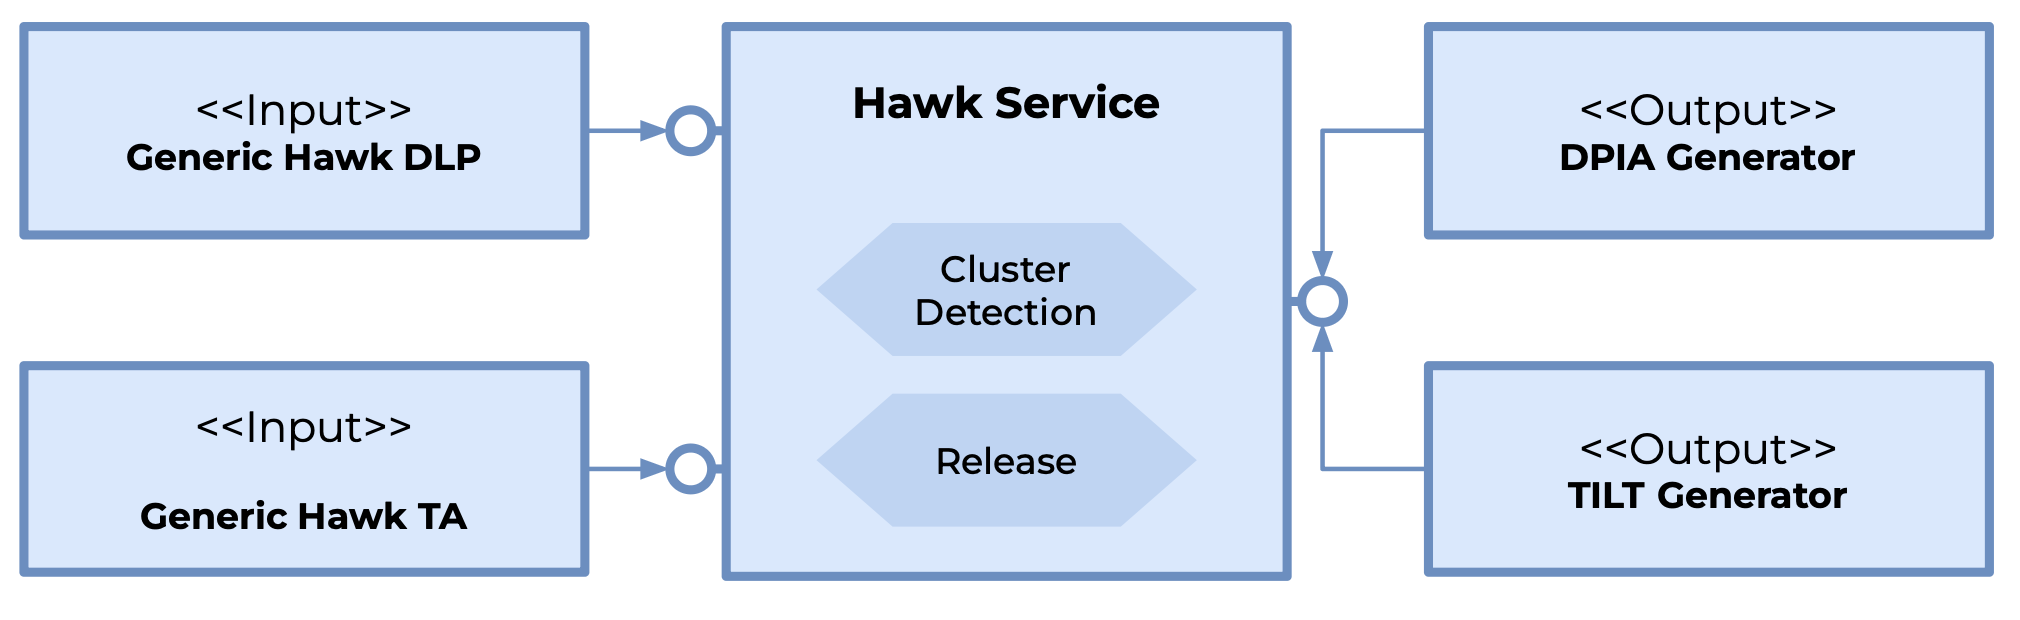
\includegraphics[width=0.95\columnwidth]{hawk-new.png}
  \caption[New Hawk Contributions]{Contributions of the new Hawk}
  \label{fig:hawk-new}
\end{figure}

\section{Hawk DLP}

The first contribution is implementing the concept of inputs and input abstractions.
It can be found on GitHub at \url{https://github.com/PrivacyEngineering/hawk-dlp}.

\begin{figure}[!h]
  \centering
  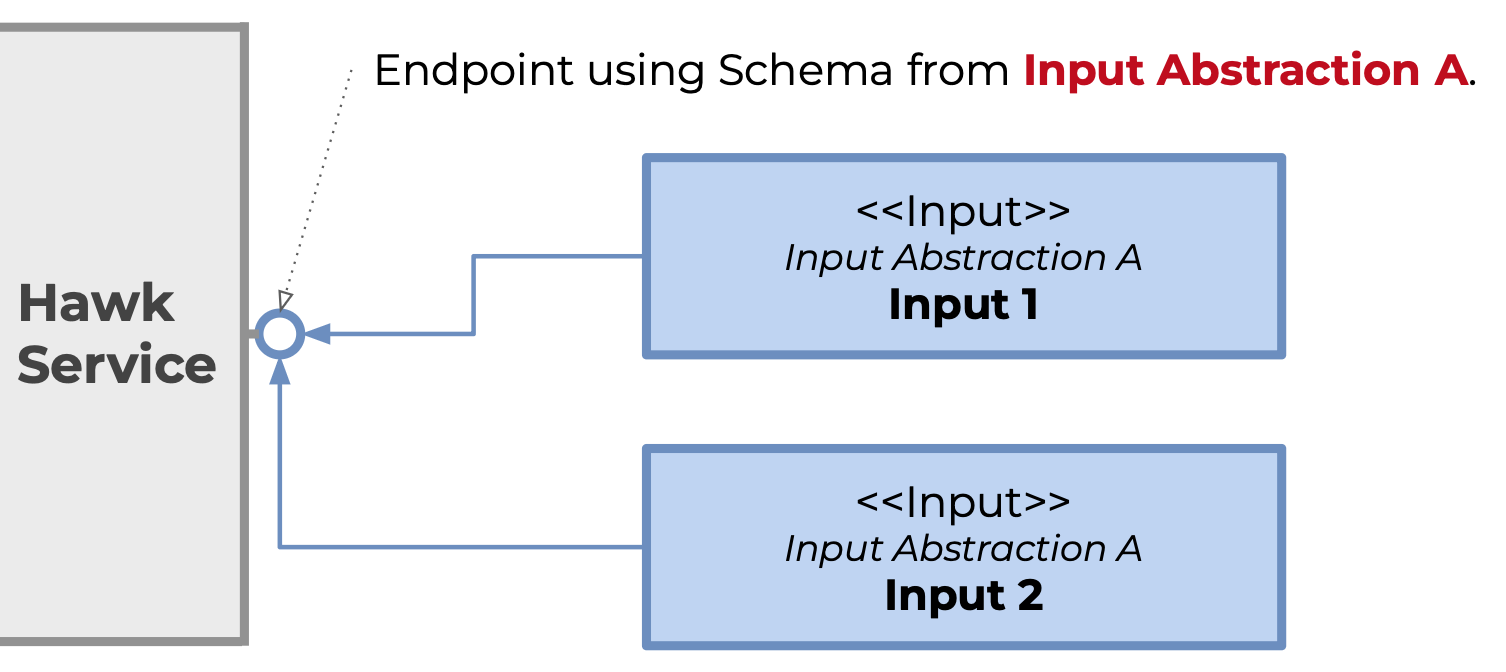
\includegraphics[width=0.95\columnwidth]{input.png}
  \caption[Input Abstractions \& Inputs]{Concept of Input Abstractions and Inputs}
  \label{fig:input}
\end{figure}

The already present integration module now works as an input for the traffic analysis input abstraction. 
Besides that, an input abstraction for DLP will be added. For this to happen, an input abstraction and some vendor-specific inputs will be added. All of this is realized in the Hawk DLP project.

\begin{figure}[!htb]
  \centering

  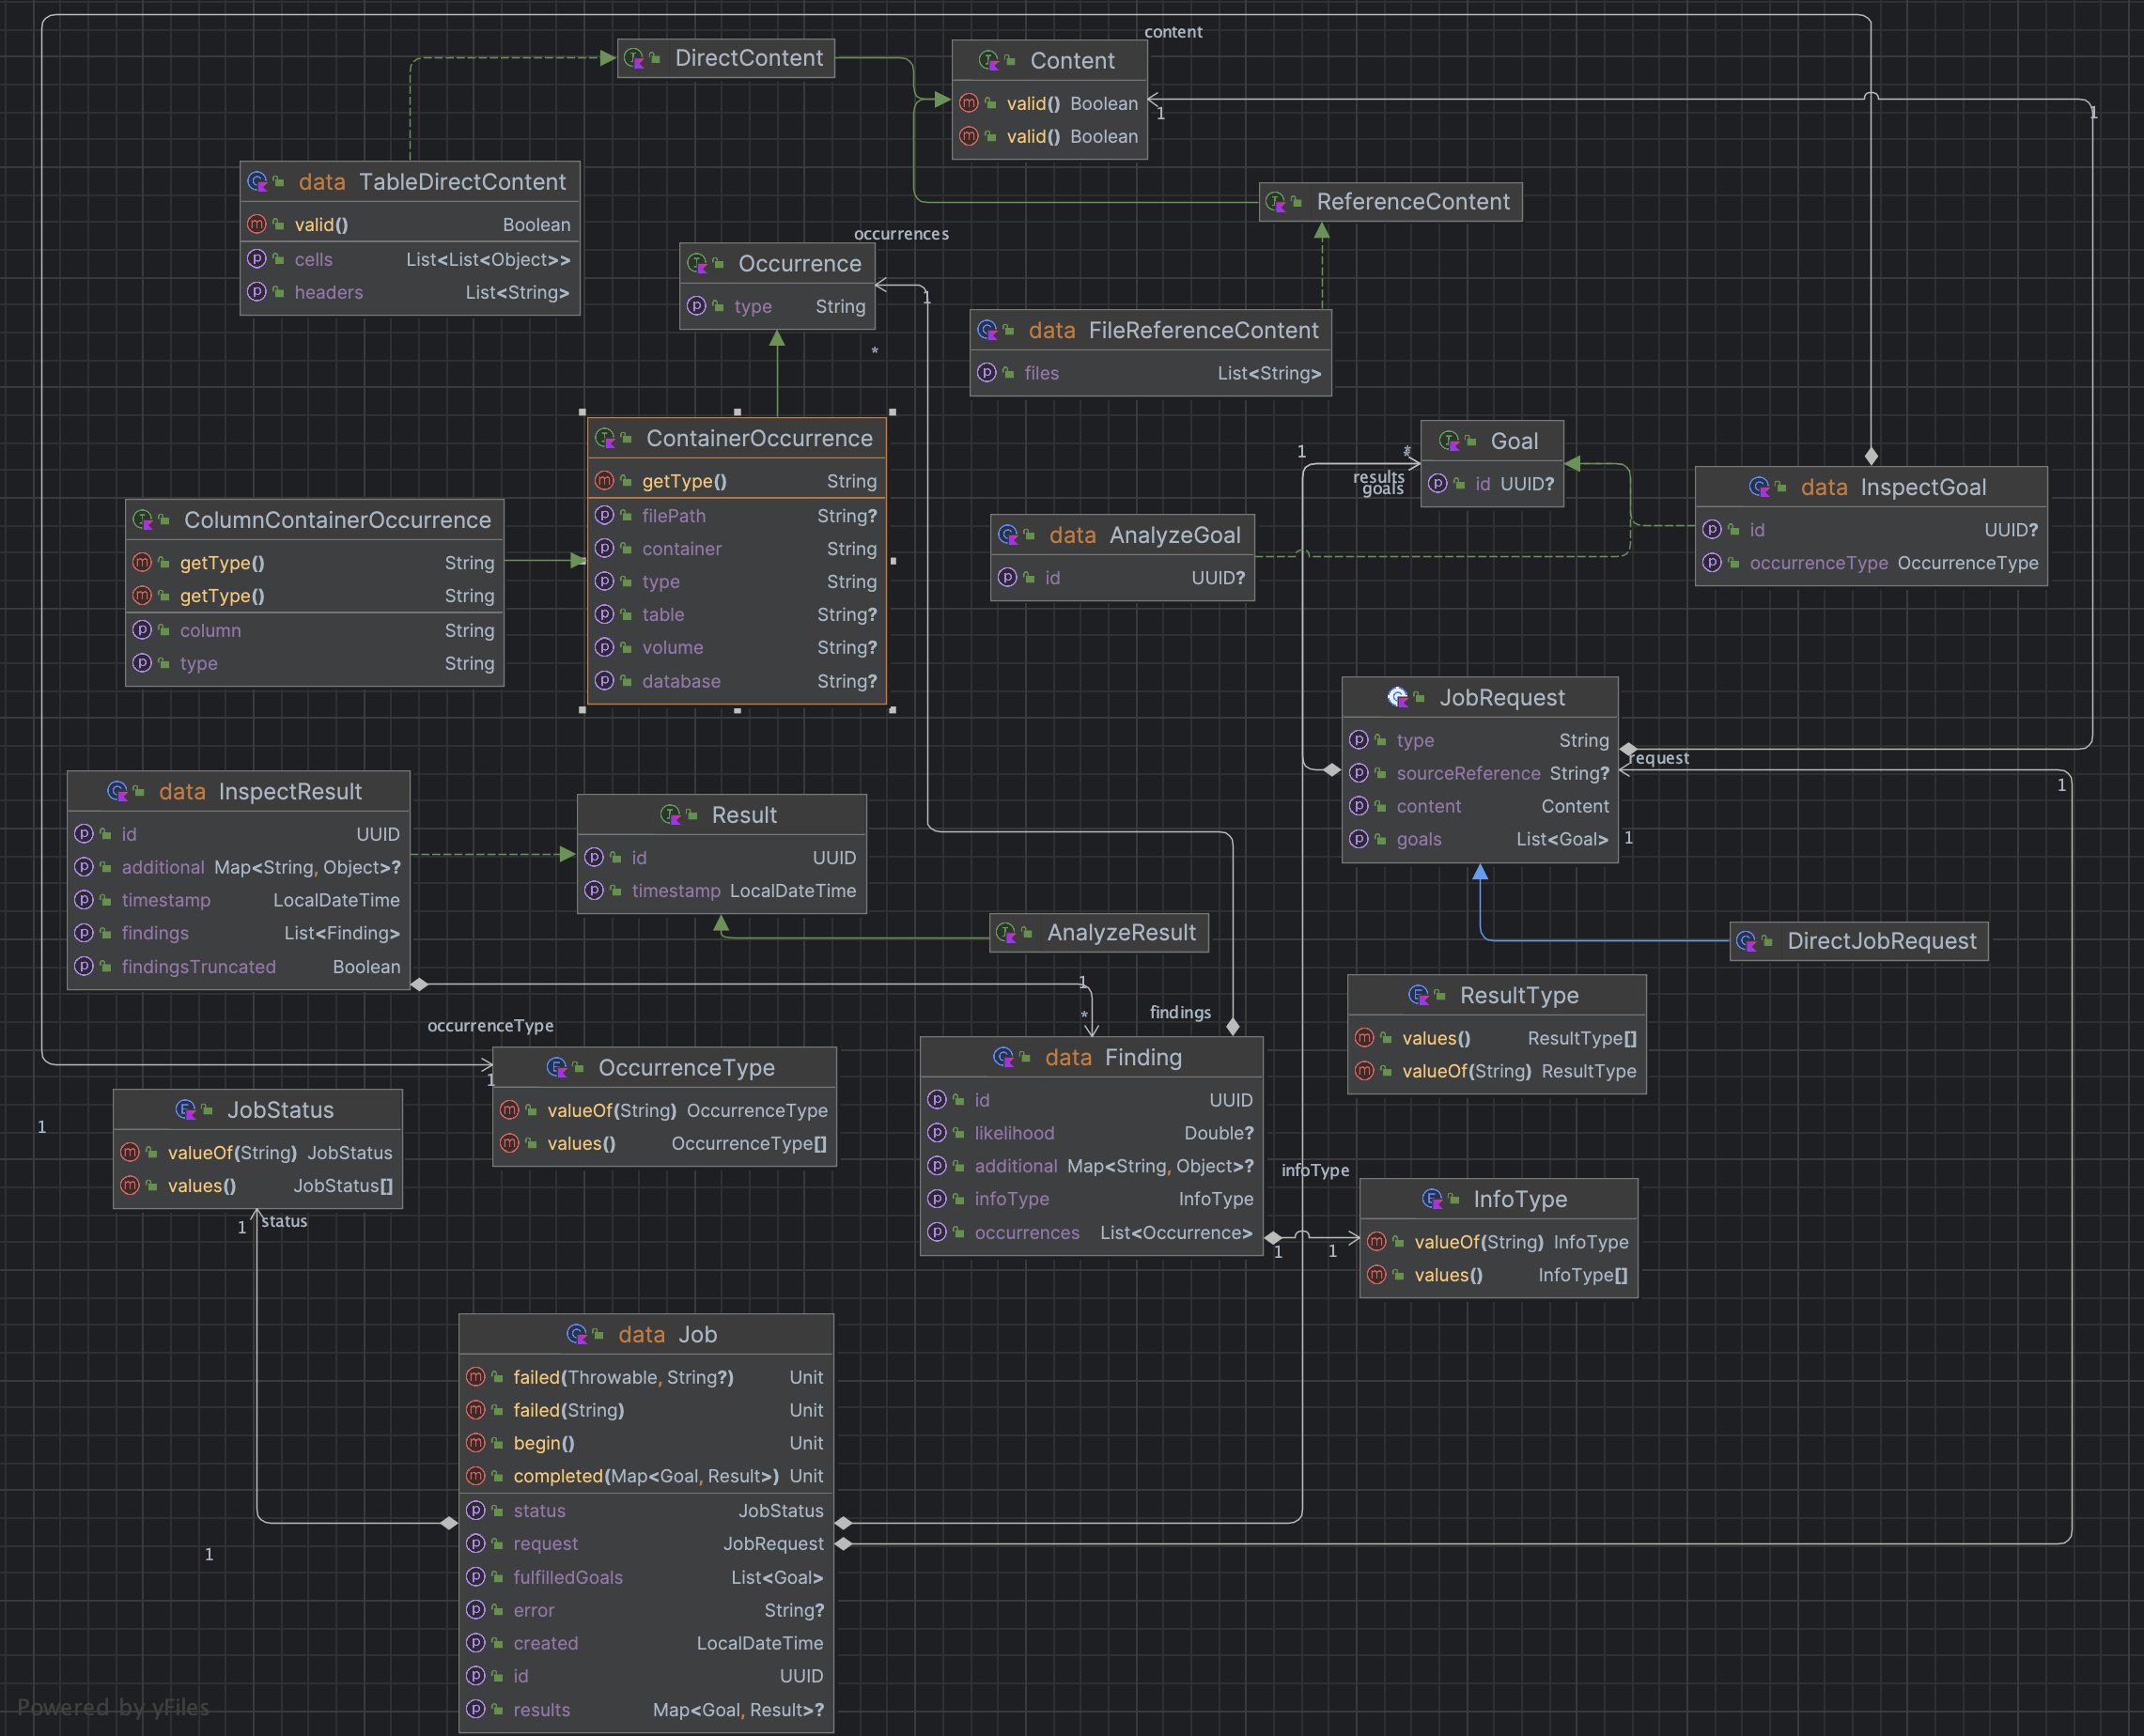
\includegraphics[width=0.95\columnwidth]{hawk-dlp-uml.png}

  \caption[Hawk DLP UML]{UML-Diagram of classes in Hawk DLP project}  
  \label{fig:hawk-dlp-uml}
\end{figure}

\subsubsection{Job}
Since the Hawk DLP input abstraction aims at abstracting DLP tools, are core concept to adapt is Jobs.
This means a job needs to be created and continuously queried until the results are present. In both cases, such a job needs to contain a reference to the data/content that should be processed and in some cases additional metadata like a goal. Besides asynchronous Jobs,
CDLP also allows embedding data directly in the request, which then gets executed synchronously.

To better explain the structure, we first look at the internal requirements for the project again. The main idea is to build a vendor-independent abstraction above standard Data Loss Prevention technologies. The first step is to build a uniform API, which other applications can use to trigger vendor-specific jobs and access the results in a common way. This uniform API is also called input abstraction. The second step is implementing the API for different Data Loss Prevention technologies, such as AWS Macie and Google CDLP.

The hawk-dlp-common and hawk-dlp-integration modules represent the input abstraction, with the common module providing the schema and the integration module providing the API.

To focus on the hawk-dlp-common module again, the first step to implementing these asynchronous jobs is to build a job abstraction for Hawk DLP. To define the term clearly, a Job represents a not yet started, a started, or a completed/failed list of tasks. Such a task is a task in the underlying DLP implementation. Note: Do not confuse Hawk DLP jobs with Macie/CDLP jobs.

Jobs can be of different types. In the code, a Job type is represented by the type of the \texttt{JobRequest}, which is also stored as a property in the job class and contains the initial parameters entered by the user to initiate the Job. The common job type, and for now the only implemented job type is the direct job, represented by the \texttt{DirectJobRequest}. A direct job is as the name suggests a job that gets executed directly and only once after creating the job. The reason for the abstraction is to have the ability to implement other job types in the future. Other job types could include a scheduled job that gets executed periodically or a trigger-based job for example. The job type name is also present in the \texttt{type} property.

Besides the job type, a job has an id property to uniquely identify the job, a creation date, and a status property. The status property is of type \texttt{JobStatus}, which is an enum and has the following allowed values: 

\textbf{CREATED} is the default status and is present right after the job creation.

\textbf{IN\_PROGRESS} is set when the Hawk DLP Integration starts processing the job.

\textbf{COMPLETED} is set when the job is finished successfully. In this case, the (final) result property is present, which will be described later.

\textbf{FAILED} is set when the processing of the job failed. In this case, a (final) error message in the error property is present.

\textit{final} that the property will not be changed in the status.

\subsubsection{Job Creation}

We will now take a deeper look at the \texttt{request} property again, which contains the initial job data provided by the user, that the integration modules use to create the job.
As the \texttt{DirectJobRequest} does not add any new properties and the \texttt{JobRequest} class is the superclass of all other job types, we will take a look at the properties of the \texttt{JobRequest} class itself.

The \texttt{content} property can be separated into \texttt{DirectContent} and \texttt{ReferenceContent}, where both classes implement the \texttt{Content} interface. \texttt{DirectContent}, not to be confused with \texttt{DirectJobRequest}, describes the content that is given directly/embedded with the job request (no matter the type of job request). Its size is often restricted due to request/body size limits etc. One concrete example of \texttt{DirectContent} is \texttt{TableDirectContent}, which represents a table that is passed along directly. It is projected by a list of column names and a two-dimensional list of table cells containing the respective value. \texttt{ReferenceContent} describes the content, which only holds a reference to the content that should be processed. An example here is \texttt{FileReferenceContent}, which contains a reference to a file or a list of files in an e.g., storage bucket.
For now, only the upper mentioned content types exist, with the abstractions in mind to make it possible to add different types of content in the future. For example, it might be interesting to add a \texttt{TableReferenceContent} in the future to represent content in databases.

The \texttt{goals} property contains a list of \texttt{Goal}s. Each goal specifies the anticipated format of the outcome/result of the job being executed. The property allows one job to have multiple results by having multiple goals in the goals list. More on that later.

Finally, the \texttt{sourceReference} property of the \texttt{JobRequest} class contains a user-set string that marks the origin of the data being processed. In the case of direct content, for example, it might not be clear from the outside where the content that is processed came from. But also for reference content, it is sometimes helpful, e.g., when aggregated data gets processed. The property is important for the Hawk Service in the next section.

\subsubsection{Job Execution}

With the \texttt{JobRequest} and the process of representing the job creation in the code explained, the next step is to explain the job execution and the way outcomes/results are represented. In the code, the instance of the job object gets forwarded to the integration. The integration then mutates the job instance and updates the \texttt{status}, \texttt{results}, and \texttt{error} properties. As explained above, right when the integration starts processing the job, the \texttt{status} property is set to \texttt{CREATED}.

To understand how the results are represented in the code, it is important to understand what the results of the DLP tools look like. Many DLP technologies share a similar set of features, where each feature works by providing input data and extracting the result after execution. With one of those being the so-called inspection feature. As explained earlier, it works by inspecting data, like for example tables and returns where which type of data was identified, e.g., column x in table y is of data type email. Another feature supported by some DLP tools is analyzation, which extracts specific privacy metrics.

Since Hawk DLP builds above other DLP tools, those features must be somehow represented. For this reason, we have the \texttt{Goal} interface and \texttt{Result} interface, with subtypes of those representing a specific DLP feature. The goal represents a feature-specific list of parameters on how to perform the feature and format the result afterward. It is provided in the job creation process, alongside the \texttt{Content} that should be processed. When processing is done, depending on the list of goals provided and whether the DLP implementation supports it, each goal gets a result associated with it.

As mentioned earlier, the main feature that we want to support is the data inspection feature. It is implemented by the \texttt{InspectGoal} and \texttt{InspectResult} classes. The feature works by inspecting the content provided and returning a list of findings, where what type of data can be found. Such a type of data could be \texttt{EMAIL}, which is represented in the \texttt{InfoType} enum. Besides the info type, some DLP implementations also give a probability that this info type is accurate. Hawk DLP represents this by a double between 0 and 1, where one is very likely. The location where the info type was found in the supplied \texttt{Content} is represented by sub-types of the \texttt{Occurrence} interface. 


There is a particular relation between the \texttt{Content} sub-type supplied, and the \texttt{Occurrence} sub-type returned. For table-based content, there is the \texttt{ColumnContainerOccurrence}. For document-based content, another sub-type could be created in the future. The \texttt{ColumnContainerOccurrence} is based on the \texttt{ContainerOccurrence}, which contains a locator for the file, database table, etc. of the finding. To create a vendor-independent interface, this interface specifies some other properties. 
For file occurrences, the \texttt{volume} and \texttt{filePath} properties are presented. The first describes the location where the file (system) of the file is located at. E.g., the name of a storage bucket. The latter describes the path of the file in the respective volume.
For (managed) database occurrences, \texttt{database} and \texttt{table} properties are present. The \texttt{database} property describes all the prefixes of the table itself. This could be a project name, depending on the database a database name and/or a schema, etc. The \texttt{table} property simply describes the table's name.
As earlier mentioned, table content has a specific type of occurrence - \texttt{ColumnContainerOccurence}. They inherit all properties from the \texttt{ContainerOccurence} and a \texttt{column} property for the column in the managed database / (CSV) file etc.
In the future, it is possible also to add a \texttt{CellContainerOccurence}, which could contain a row identifier besides the column name and allow for a cell-specific inspection of the data.

To reduce redundant data, occurrences with the same info type (and if present likelihood) get aggregated in the same finding. Meaning a finding has a list of occurrences. The \texttt{InspectResult} simply contains a list of \texttt{Finding}s and a boolean, whether any findings were excluded or not (some might be excluded because of size limits etc.). Depending on the implementation some additional properties might exist in the \texttt{InspectResult}, \texttt{Finding}, and/or \texttt{Occurrence} classes. To transform the result from the DLP implementation, it is required to specify the \texttt{OccurrenceType} in the \texttt{InspectGoal}.

A second feature, which is not yet implemented but is supported by some DLP technologies is the analyzation feature. It calculates specific privacy metrics from the data supplied. For future implementation, the \texttt{AnalyzeGoal} and \texttt{AnalyzeResult} classes were already added.

To enable multiple types of results by one execution, the \texttt{JobRequest} gives the possibility to specify multiple \texttt{Goal}s in the request. This results in one \texttt{Result} being created for each \texttt{Goal}.

Now, back to the job execution process. Job Status is changed to \texttt{IN\_PROGRESS} when the request was passed to the integration. The integration extracts the request and passes the data to the DLP implementation. When the DLP implementation responds with a result, the integration parses it according to the \texttt{Goal}s provided and fills the \texttt{results} map in the \texttt{Job} class. In this case, the \texttt{JobStatus} gets updated to \texttt{COMPLETED}. In case of an error, the \texttt{FAILED} \texttt{JobStatus} is set, and their error messages are saved in the \texttt{error} property.

\subsection{Integration Module}

The integration module simply adds a base module for all integrations. Since integration modules expose a uniform REST API and use the Spring Boot Framework, it abstracts the presentation layer (according to Domain-Driven-Design \cite{millett_patterns_2015}) and provides some interface for an extension. The integration module depends on the common module and uses its types for abstraction. 

\paragraph{REST API}
Different endpoints are defined in the \texttt{JobController}. All of them provide CRUD-based operations for the Job entity or any of its sub-entities.

The first category of endpoints is used to create jobs. As described in the common module, different Job types exist. In the API this is represented by one endpoint per Job type. Currently, only one Job type exists - the direct job type. This means that the only endpoint is the \texttt{direct job create} endpoint. It is accessible under \texttt{POST /api/v1/jobs/direct}. As a request body, a \texttt{DirectJobRequest} must be provided as JSON. When the input is valid, a \texttt{Job} instance will be returned.

The second endpoint is to list all cached \texttt{Job}s. Each instance of the Hawk DLP integration stores a list of that are/were processed by it. Currently, this list is volatile. In the future, this could be easily implemented with persistence to enable browsing older jobs and achieve horizontal scalability of Hawk DLP integration instances. The endpoint is accessible under \texttt{GET /api/v1/jobs}

To inspect single job instances, the \texttt{GET /api/v1/jobs/\{id\}} endpoint can be used. The path variable \texttt{id} represents the \texttt{id} property of the \texttt{Job} class returned by a job create endpoint. This endpoint should be used to access completed jobs and/or monitor jobs in progress.

Since some properties are suppressed in the JSON view of the \texttt{Job} due to their size, some get endpoint for the sub-entities of the \texttt{Job} class exists.
Namely, the \texttt{request} and the \texttt{results} properties are suppressed. The first can be accessed by \texttt{/request} as a suffix - \texttt{GET /api/v1/jobs/\{id\}/request}. The latter represents a list of results. Therefore, the \texttt{GET /api/v1/jobs/\{id\}/results} endpoint only returns a list of result ids available to this job. By specifying the result id in \texttt{GET /api/v1/jobs/\{id\}/results/\{resultId\}}, the individual \texttt{Result} can be accessed.

\subsubsection{Job API}

To forward requests of the REST API to the concrete integration implementation, an abstraction is provided. The \texttt{JobService} class holds a \texttt{Map} of stored jobs by this Hawk DLP integration instance. When an endpoint is called, the response is served by accessing or modifying this \texttt{Map}. Besides adding a Map-Entry when creating a job via. any of the job create endpoints, a Spring event is published in the Spring \texttt{EventBus}. Integration implementations can listen to the \texttt{JobCreatedEvent} being published in the Event bus, holding the \texttt{Job} instance and start processing the request. The \texttt{Job} instance will be mutated by the Integration implementation, which leads to the endpoints immediately serving the new content.

\section{Hawk API \& Hawk Service}

It can be found on GitHub at \url{https://github.com/PrivacyEngineering/hawk-service/tree/feature/v2}.

\begin{figure}[!htb]
  \centering

  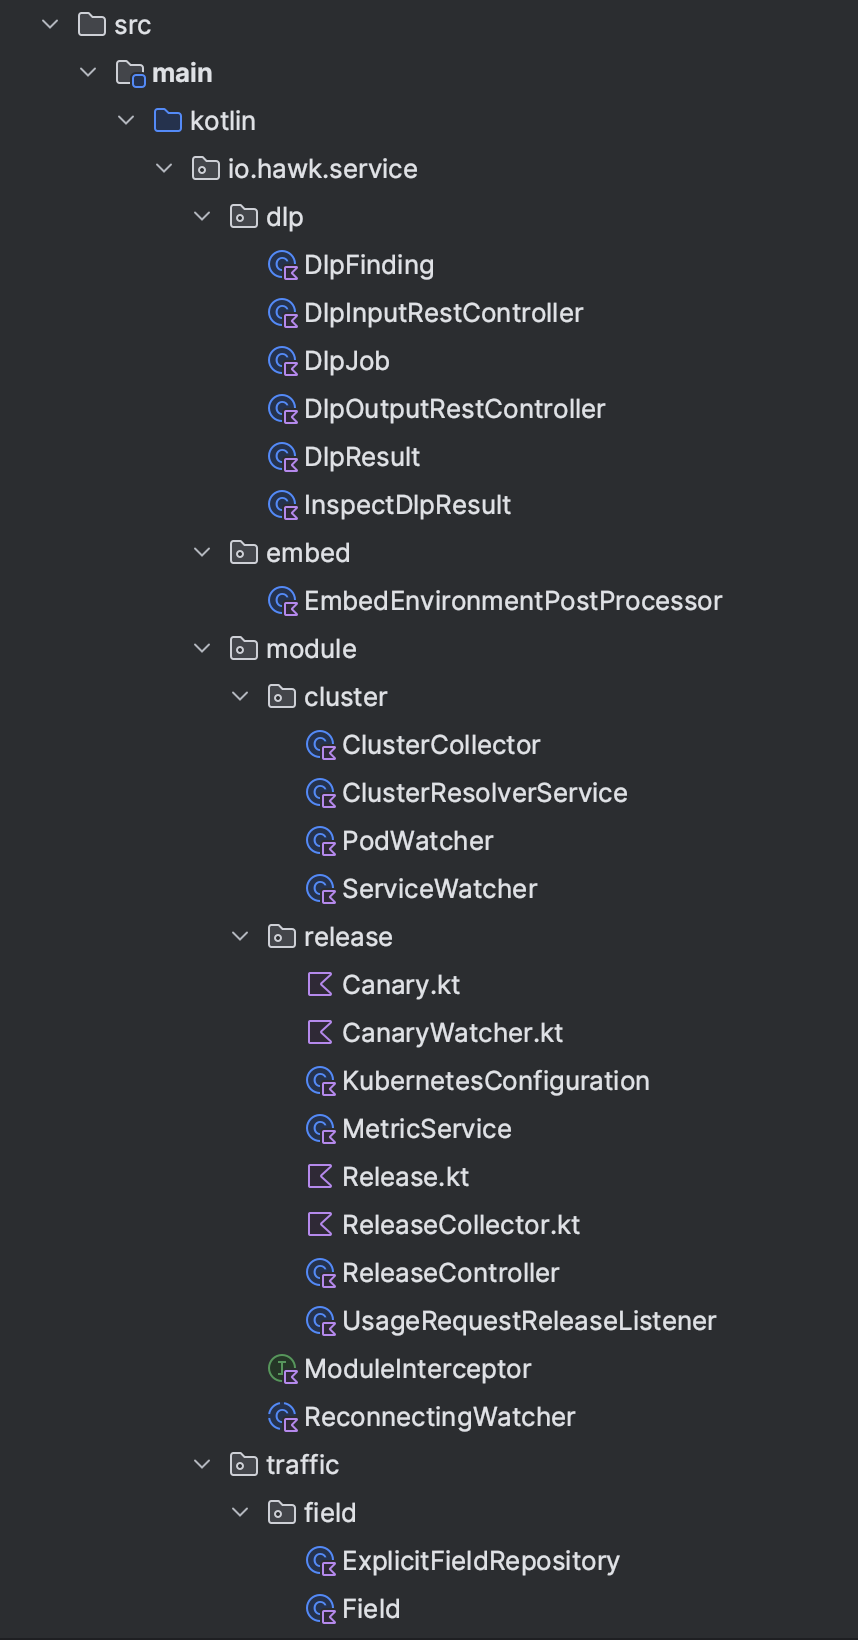
\includegraphics[width=0.8\columnwidth]{hawk-service-file.png}

  \caption[Hawk Service file structure]{Filestructure of Hawk Service project showing Domain-Driven-Design}  
  \label{fig:hawk-dlp-uml}
\end{figure}
Like the original version of Hawk, the Hawk Service is a core component of the Hawk Framework. It serves the Hawk API, which can be used to access data from the technologies behind Hawk uniformly. One of the main contributions to the Hawk Service is the encapsulation of inputs and outputs. The project still follows a strict package-by-feature layout but with all the old classes grouped into a traffic-analysis package. The release module is encapsulated into a \texttt{module/release} package. Along with it, some module classes themselves were abstracted to be reused in other modules.

\subsection{Hawk DLP integration}
To enable the Hawk API to return information extracted via DLP tools, Hawk DLP inputs have to communicate with the Hawk Service. This communication works by letting the Hawk API expose a Hawk-DLP-Job-Update endpoint. This endpoint receives Hawk DLP Jobs parses them with available internal modules and then persists those changes into a database. Using the data persisted in this database, the Hawk API can access all saved jobs.

The transmission of the DLP-Jobs can be optionally enabled in the Hawk DLP input. By default, it is disabled to have the ability to run Hawk DLP autonomously. 
In detail, this was realized by having the integration module of the Hawk DLP project provide an interceptor that can be enabled to send all Job updates to the Hawk Service. In this case, the REST-API of the Hawk DLP input still works normally. The push-based approach of pushing Job-update to the Hawk Service is to enable running multiple different Hawk DLP inputs without registering each one at the Hawk Service. Alternatively, a pull-based approach would be possible, bringing the challenge of coordinating Job-Update-Reqeuests when having multiple Hawk Service instances running. Using the push-based approach, the only stateful component is the database, which makes the whole application horizontally scalable and cloud-native.

\subsection{Hawk Cluster detection module}
Another new contribution of the new Hawk Service is the Cluster detection module.
As mentioned above, many companies today are using microservices. The idea of a microservice is to handle a small part of a bigger application. A core requirement of the microservice architecture is encapsulation, which results in many microservices having their own (private) components, such as databases, etc. Since there is no completely accurate way of identifying to which microservice a database belongs, the Hawk Cluster detection module introduces a \texttt{hawk.io/app-name} label. This label is only available in Kubernetes-based environments.

The cluster detection module works by resolving the label mentioned above from the component present in the context. In the case of a DLP Job, such a context could be the \texttt{JobRequest.sourceReference} property. In the case of traffic analysis, which is already present in the old Hawk Framework, it could \texttt{Usage.endpointHost}. The cluster detection module then uses the Kubernetes API to identify \texttt{Pod}s, \texttt{Service}s, \texttt{EndpointSlice}s or the current \texttt{Namespace} from the context to resolve the label value. The cluster detection module then tags the DLP Jobs / Traffic-Analysis Processing activities with this app-name value. Based on those tags queries can be made, as explained in the next section.

\subsection{Hawk API}
As covered in previous sections, the Hawk API is a collection of new endpoints available to the Hawk Service.
Those endpoints follow the REST paradigm and are primarily grouped by their respective feature (DLP, traffic analysis, app, etc.) and secondarily by their layer (input, output). Input means endpoints where data can be inserted/created, and output means endpoints that return data. The Hawk API can therefore be separated into the following categories/features:

\subsubsection{Traffic Analysis [Input, Output]}
The traffic analysis endpoints are similar to the previous Hawk Framework, with the insert endpoint being untouched. Mainly there are two endpoints for submitting Processing activities, one for submitting in batch mode. Currently, there is no query (output) endpoint for Processing activities. However, this can be changed as the data model is available. For Fields and Mappings all Create-Read-Update-Delete (CRUD) endpoints are available.


\subsubsection{Data Loss Prevention [Input, Output]}
The new Hawk Framework also features a REST API that is similar to that of the Hawk DLP input. However, since the Jobs and Job results are persisted in the Hawk Service and tagged with metadata, some more information is available at the Hawk Service. Also, results of multiple DLP inputs can be viewed, which is helpful if, e.g., a Multi-Cloud Environment is present. The DLP API in the Hawk Service features a Job insert endpoint, typically called by the DLP inputs to submit Job changes. There is no endpoint for initiating a Job, as this needs to be done at the respective input directly.

\subsubsection{Application [Output]}
As explained in the cluster detection module section, the Hawk Service tags incoming objects, such as Processing activities or Jobs, with their respective App name extracted from the Cloud Environment. To enable the synergy effects of different input abstractions, the Hawk API offers endpoints for querying data by application name. Using these endpoints, the "complete picture" mentioned in the problem section can be achieved if enough input abstractions are present. Since this is only an aggregation of data inserted in other endpoint groups, no input endpoints are available here.

With everything implemented, the Hawk Framework will look like this:
\begin{figure}[!htb]
  \centering

  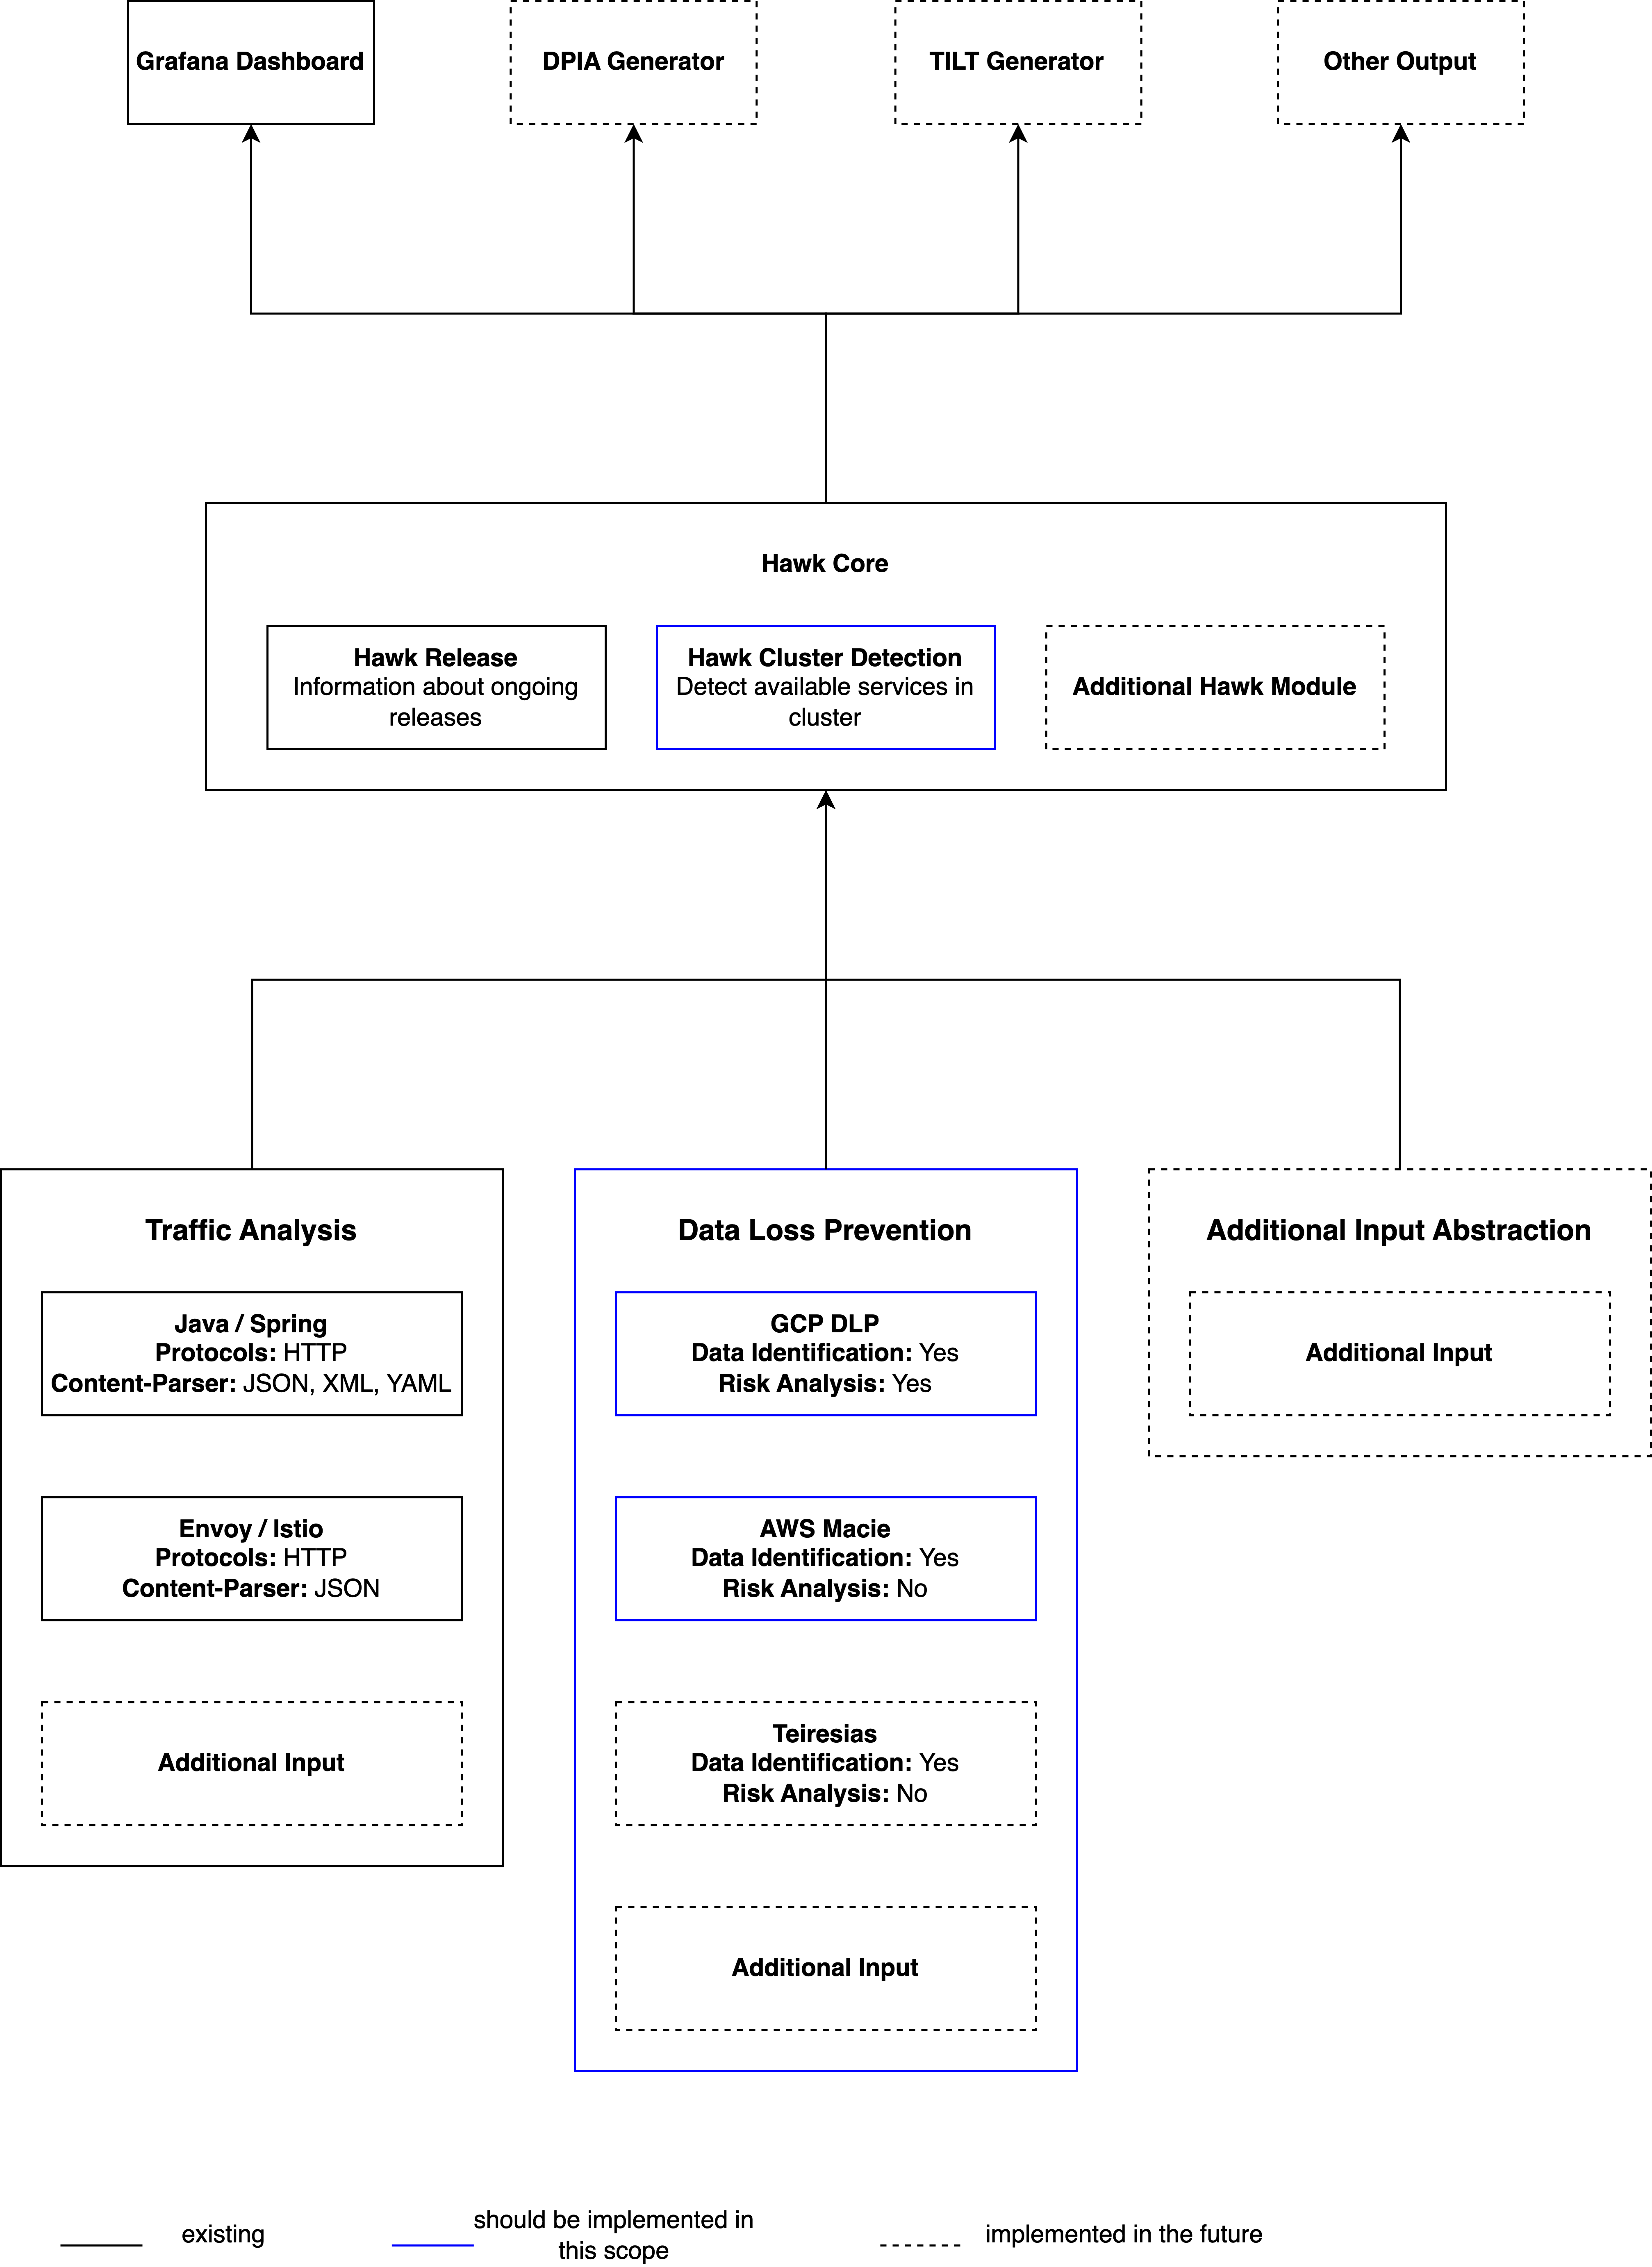
\includegraphics[width=0.95\columnwidth]{hawk.png}

  \caption[Hawk architecture]{The Hawk architecture diagram, with all the new parts, focused on this thesis marked blue.}  
  \label{fig:hawk}
\end{figure}




% ---------------------------------------------------------------------------
% ----------------------- end of thesis sub-document ------------------------
% ---------------------------------------------------------------------------